\documentclass[conference]{IEEEtran}
\IEEEoverridecommandlockouts
\usepackage{cite}
\usepackage{amsmath,amssymb,amsfonts}
\usepackage{algorithmic}
\usepackage{graphicx}
\usepackage{textcomp}
\usepackage{xcolor}
\usepackage{booktabs}
\def\BibTeX{{\rm B\kern-.05em{\sc i\kern-.025em b}\kern-.08em
    T\kern-.1667em\lower.7ex\hbox{E}\kern-.125emX}}

\begin{document}

\title{Smart Karawala: A Batch-Centric AI--IoT Framework\\
for Predictive and Automated Dry-Fish Processing}

\author{
\IEEEauthorblockN{L. B. R. V. Vivipem}
\IEEEauthorblockA{\textit{Dept. of Information Technology}\\
\textit{SLIIT}, Malabe, Sri Lanka\\
email or ORCID}
\and
\IEEEauthorblockN{E. W. M. Sanjaya}
\IEEEauthorblockA{\textit{Dept. of Information Technology}\\
\textit{SLIIT}, Malabe, Sri Lanka\\
email or ORCID}
\and
\IEEEauthorblockN{G. A. K. J. Peshala}
\IEEEauthorblockA{\textit{Dept. of Information Technology}\\
\textit{SLIIT}, Malabe, Sri Lanka\\
email or ORCID}
\and
\IEEEauthorblockN{D. T. C. D. P. Gunasekara}
\IEEEauthorblockA{\textit{Dept. of Information Technology}\\
\textit{SLIIT}, Malabe, Sri Lanka\\
email or ORCID}
\and
\IEEEauthorblockN{[Supervisor]}
\IEEEauthorblockA{\textit{Dept. of Information Technology}\\
\textit{SLIIT}, Malabe, Sri Lanka\\
email or ORCID}
\and
\IEEEauthorblockN{[Co-Supervisor]}
\IEEEauthorblockA{\textit{Dept. of Information Technology}\\
\textit{SLIIT}, Malabe, Sri Lanka\\
email or ORCID}
}

\maketitle

\begin{abstract}
Small-scale dry-fish processing in Sri Lanka depends on operator experience
and open-air drying, producing inconsistent quality, spoilage risk, and
fragmented batch histories. Existing work treats environmental monitoring,
machine-learning drying prediction, process control, and traceability as
separate functions, and rarely returns a prediction to the drying equipment
as an operating set-point. This paper presents Smart Karawala, a
batch-centric Artificial Intelligence (AI) and Internet of Things (IoT)
framework that links these functions in one processing lifecycle. A unique
batch identifier ties preparation data, continuous temperature, humidity,
gas and weight sensing, machine-learning prediction of the drying
temperature and duration, rule-based spoilage- and over-drying-risk
assessment, automated drying control, and sustainability records. A
two-phase start protocol turns the predicted parameters into the chamber's
control profile and records a batch as drying only after the chamber
confirms a valid sensor state, and an independent safety layer clamps every
set-point and can stop the heater regardless of the model. On a
physics-informed modelled drying dataset the remaining-time regressor
reached a grouped cross-validated coefficient of determination of 0.96
(mean absolute error 1.1 min). We report the integration status of each
subsystem and the field experiments still required.
\end{abstract}

\begin{IEEEkeywords}
artificial intelligence, cyber-physical systems, dry-fish processing,
Internet of Things, machine learning, process control, traceability
\end{IEEEkeywords}

\section{Introduction}
Drying preserves food by reducing available moisture, suppressing microbial
and enzymatic activity. In Sri Lanka roughly a quarter of the marine fish
harvest is dried, and dried fish (\emph{karawala}) supports coastal
livelihoods; reported post-harvest quality losses in the sector are high,
and open-sun drying is associated with spoilage, contamination, and
weather-dependent inconsistency~\cite{b12}. Processing remains manual:
operators judge cleaning losses, salt quantity, salting duration, drying
conditions, and final dryness from experience, while open yards expose the
batch to changing temperature and humidity.

IoT, machine learning (ML), and closed-loop control can replace
experience-dependent judgement with data-driven workflows, but implemented
in isolation their combined value is limited. A drying-time estimate is
more useful when continuously updated from live readings; a control
decision is more defensible when its evidence is retained against the batch
record. A recent review identifies closed-loop integration of sensing,
prediction, and control as an open direction~\cite{b3}.

This paper presents \emph{Smart Karawala}, which treats preparation,
sensing, prediction, control, verification, and traceability as stages of
one lifecycle. A batch is observed through
\begin{equation}
X(t) = [\,T(t),\ H(t),\ W(t),\ G(t),\ B\,],\label{eq1}
\end{equation}
where $T,H,W,G$ are chamber temperature, relative humidity, batch weight,
and a gas/odour signal, and $B$ is batch preparation data. These support
\begin{equation}
Y(t) = [\,\hat{\theta},\ \hat{R}_{0},\ \hat{R}(t),\ P_{s}(t),\ U(t),\
D(t)\,],\label{eq2}
\end{equation}
where $\hat{\theta}$ is the recommended chamber temperature, $\hat{R}_{0}$
the predicted total drying time, $\hat{R}(t)$ the re-estimated remaining
time, $P_{s}(t)$ a spoilage-risk level, $U(t)$ control actions, and
$D(t)$ the completion state.

\textit{Contribution.} The central contribution is a batch-centric
cyber-physical architecture that passes ML drying predictions into an
IoT-controlled drying chamber while an independent safety layer can
override the predictive path, and retains every decision as an event-level
batch history. Secondary contributions are: (i) a two-phase
prediction-to-control handoff in which a batch is recorded as drying only
after the chamber independently confirms a valid sensor state; (ii)
grouped-cross-validated remaining-time prediction; (iii) sensor-fault and
over-drying protection independent of model output; and (iv) a reported
integration failure mode -- a service holding a \emph{logical} record of
drying must not be treated as authoritative about whether drying is
\emph{physically} occurring. The research question is whether integrating
heterogeneous sensing, prediction, and automated control provides a
coherent, safe framework for digitising small-scale dry-fish processing.

\section{Related Work}
\textbf{IoT and drying control.} Mishra \textit{et al.}~\cite{b1} showed
that real-time measurement and actuation stabilise food drying; Alvinika
\textit{et al.}~\cite{b2} regulated a fish-drying chamber from temperature
and humidity with fuzzy logic on low-cost hardware. Such systems measure
the drying \emph{environment} rather than the product state, and many
remain reactive~\cite{b3}.

\textbf{ML for drying prediction.} For an observation sequence
$X_{1:t}$, a regressor estimates the remaining time as
$\hat{R}_{t} = f(X_{1:t})$. Rakholia \textit{et al.}~\cite{b4} predicted
meat drying time from process history for production planning; Ahmad
\textit{et al.}~\cite{b5} estimated grain moisture from environmental
parameters. Thin-layer models remain the physical baseline; Ghanem
\textit{et al.}~\cite{b6} fitted them to solar-dried salted tilapia with
close agreement to measured moisture ratios. Predictions are typically
advisory, and few systems return a predicted parameter to the equipment as
a control set-point.

\textbf{Freshness sensing and traceability.} Setyagraha \textit{et
al.}~\cite{b8} discriminated seafood freshness with low-cost metal-oxide
gas sensors and ML classifiers, supporting an inexpensive gas sensor as an
odour proxy. Cromwell \textit{et al.}~\cite{b10} reviewed digital fish
traceability and identified integration as a prerequisite for higher
traceability levels; Tsang \textit{et al.}~\cite{b11} demonstrated a
blockchain--IoT architecture for perishable-food traceability. This work
concentrates on catch and distribution, treating processing as one opaque
event.

\textbf{Research gap.} Each function above contributes individually.
Predictive models are usually evaluated in isolation rather than used to
set equipment parameters; drying temperature is usually a fixed operator
input rather than a predicted quantity; and traceability research records
supply-chain custody rather than the decisions taken \emph{during}
processing.

\section{Proposed Integrated Framework}

\subsection{Architecture and Batch-Centric Data Model}
Smart Karawala is organised around the lifecycle of one batch
(Fig.~\ref{fig1}). It comprises four loosely coupled services over HTTP
with a document store, plus a cross-platform mobile application: an
authentication service; a batch and sustainability service that owns batch
data, cleaning-loss and salt estimation, salting progression, waste
records, and traceability reporting; an environmental-monitoring service
that runs the drying-chamber state machine and actuator control at the
edge; and a predictive-analytics service that produces the ML predictions
and rule-based risk assessments and orchestrates drying. Each batch has a
record
\begin{equation}
B_{i} = \{\,P_{i},\ E_{i},\ W_{i},\ A_{i},\ S_{i},\ T_{i}\,\},\label{eq3}
\end{equation}
with preparation data $P_{i}$, environmental observations $E_{i}$, weight
progression $W_{i}$, analytical outputs $A_{i}$, sustainability data
$S_{i}$, and processing/traceability events $T_{i}$. The analytics service
reads batch data and live readings only over the other services' public
interfaces, so no service touches another's database.

\subsection{End-to-End Workflow}
The framework follows a \emph{sense--predict--decide--control--verify--%
trace} cycle (Fig.~\ref{fig2}). A batch is created with its variety and raw
weight; cleaning loss and salt requirement are estimated and the batch is
salted, with drying gated until salting is recorded complete. Before
drying, the analytics service predicts the recommended temperature and
total time; those values are registered with the chamber as a control
profile; the chamber validates its own sensors and starts; only then does
the analytics service record the batch as the single active drying batch.
During drying, a periodic loop pulls the latest reading, re-estimates the
remaining time, evaluates spoilage and over-drying risk, and -- at high
over-drying risk -- stops the heater. Completion is detected from weight
and elapsed time, the chamber runs a cooling phase, and every significant
event is written against the batch identifier.

\begin{figure}[t]
\centering
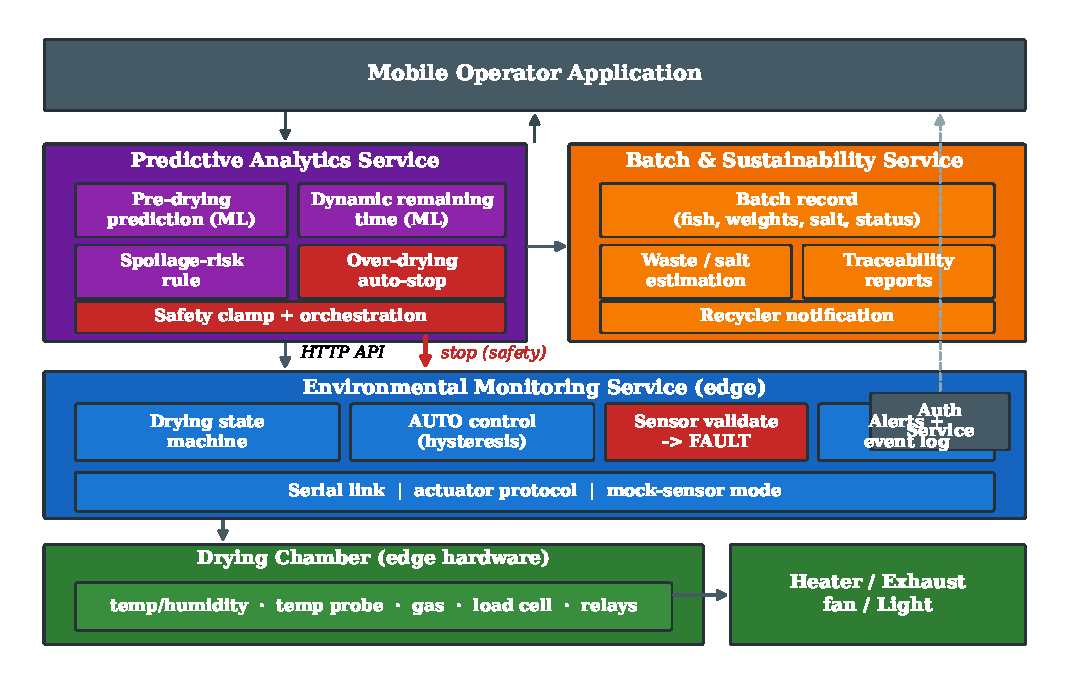
\includegraphics[width=\columnwidth]{fig1_architecture.pdf}
\caption{System architecture. The monitoring service holds the edge
controller, sensors, and relays; the analytics service holds the ML
predictors and the safety and orchestration logic; the batch service owns
the batch record. Solid arrows are HTTP calls; the safety auto-stop path
is highlighted.}
\label{fig1}
\end{figure}

\begin{figure}[t]
\centering
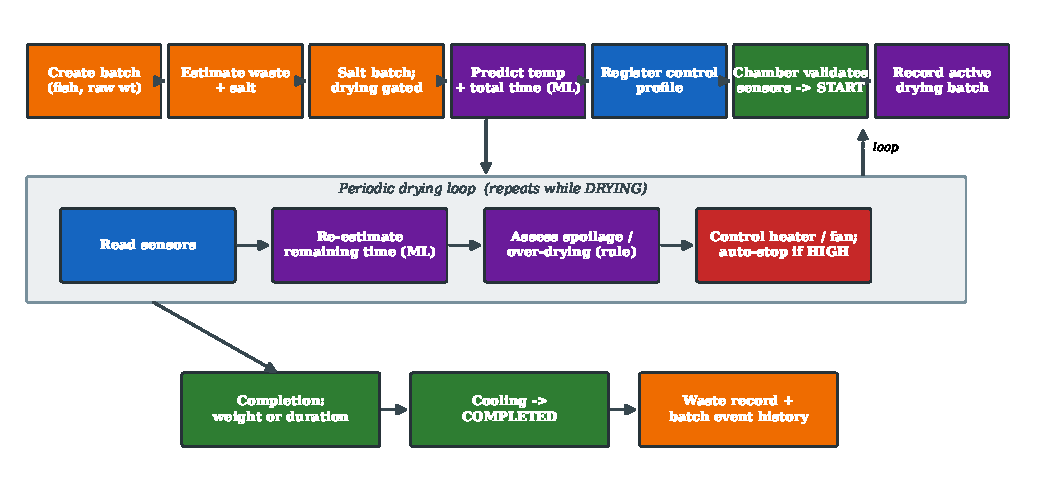
\includegraphics[width=0.86\columnwidth]{fig2_workflow.pdf}
\caption{End-to-end batch workflow: creation, salting, the two-phase
drying start, the periodic drying loop, completion verification, and the
batch event history.}
\label{fig2}
\end{figure}

\section{Monitoring and Predictive Processing}

\subsection{Environmental and Physical Sensing}
An edge microcontroller streams a periodic sensor block over a serial link
from a temperature/humidity sensor, a temperature probe, a metal-oxide gas
sensor, and a load cell with a signal-conditioning amplifier. Malformed
lines are rejected, and a reading drives control only when every required
field is present and physically plausible. The environmental state is
$E_{t}=[\,T_{t},H_{t}\,]$, with a safe operating condition
\begin{equation}
C_{E}(t) =
\begin{cases}
1, & T_{\min}\!\le\! T_{t}\!\le\! T_{\max}\ \wedge\ H_{t}\!\le\! H_{\max}\\
0, & \text{otherwise.}
\end{cases}\label{eq4}
\end{equation}
A software-simulation mode reproduces the sensor block in the device
format, so the full system runs without hardware for development.

\subsection{Weight Progression}
From the captured initial weight $W_{0}$,
\begin{equation}
R_{W}(t)=\tfrac{W_{t}}{W_{0}},\ \
L_{W}(t)=\tfrac{W_{0}-W_{t}}{W_{0}}\!\times\!100,\ \
r_{W}(t)=\tfrac{W_{t-\Delta t}-W_{t}}{\Delta t}.\label{eq5}
\end{equation}
Because both time predictors and the completion check share this signal,
the analytics service applies a reliability gate: the weight-loss rate is
used only once enough time has passed and enough mass lost for the ratio
to clear sensor noise; until then the pre-drying estimate is shown.

\subsection{Gas Sensing}
The metal-oxide gas sensor gives an odour-related signal linked to
volatiles from protein degradation. Its raw reading is mapped to discrete
smell levels using configurable prototype thresholds; consistent
with~\cite{b8}, it is treated as an uncalibrated odour proxy, not a direct
spoilage measurement.

\subsection{Pre-Drying Parameter Prediction}
Before drying, the system predicts the recommended chamber temperature and
total drying time from conditions known in advance,
\begin{equation}
[\,\hat{\theta},\ \hat{R}_{0}\,] = f_{\phi}(\textit{variety},\ W_{0},\
H_{0},\ G_{0}).\label{eq6}
\end{equation}
Here temperature is itself predicted and in turn shapes the expected
duration, unlike approaches that fix temperature as an operator input. The
predictor is a multi-output regression ensemble, selected by
cross-validation. Where a live reading is unavailable, a documented default
is substituted and the result marked, so a sensor-grounded estimate is
distinguishable from a fallback.

\subsection{Dynamic Remaining-Time Prediction}
During drying, the feature vector is
\begin{equation}
Z_{t} = [\,\textit{variety},\ W_{0},\ W_{t},\ T_{t},\ H_{t},\ \tau_{t},\
r_{W}(t)\,],\label{eq7}
\end{equation}
with elapsed drying time $\tau_{t}$, and $\hat{R}_{t}=f_{\theta}(Z_{t})$.
The prediction is refreshed periodically; the client applies a short
rolling average and permits an upward correction only past a tolerance, so
the displayed countdown stays steady under noise.

\subsection{Rule-Based Spoilage-Risk Assessment}
Spoilage risk is a transparent weighted rule over the odour level,
humidity, temperature, and stalled weight loss:
\begin{equation}
s = \sum_{k} w_{k}\,\mathbb{1}[\,c_{k}\,],\qquad
P_{s} = \Phi(s),\label{eq8}
\end{equation}
where each $c_{k}$ is a threshold condition, $w_{k}$ its weight, and
$\Phi$ maps $s$ to Low/Medium/High. The interface reports each contributing
reading with its value, expected range, and direction of influence. This
is a rule-based risk assessment, not a trained classifier; a learned
classifier is future work, pending labelled spoilage ground truth.

\subsection{Sustainability Estimation}
At batch creation the platform estimates expected cleaning waste and the
required salt quantity and salting duration from per-variety coefficients,
storing them against the batch. Salting progress is estimated from elapsed
time against the recommended duration. A recorded waste event is
$W_{e}=\{\textit{type},\textit{quantity},\textit{time},\textit{method},BID\}$,
and a recycler-collection message is composed and stored with the batch.

\section{Decision, Control, and Traceability}

\subsection{Automated Drying Control}
The chamber runs a state machine
\textsc{ready}$\rightarrow$\textsc{drying}$\rightarrow$\textsc{cooling}%
$\rightarrow$\textsc{completed}, plus \textsc{stopped} and \textsc{fault}.
In automatic mode the heater switches with fixed hysteresis about the
target temperature and the exhaust fan responds to the humidity target;
$U_{t}=\pi(S_{t},E_{t})$ yields heater activation, fan activation,
continuation, protective intervention, or termination. Temperature and
humidity feedback influence subsequent commands, so control is closed-loop
at the controller level; physical actuator acknowledgement is not yet read
back (Section~VI).

\subsection{Independent Safety Layer}
Two properties are enforced independently of the ML path. Every recommended
temperature is clamped before it can reach the controller,
\begin{equation}
\theta_{\text{safe}} = \min\!\big(\max(\hat{\theta},\ T_{\min}),\
T_{\max}\big),\label{eq9}
\end{equation}
applied in the analytics service, again at drying start, and again on the
client; this bound is correct by construction -- an out-of-range value
cannot be forwarded. Independently, the chamber faults and de-energises the
heater after a bounded number of consecutive missing or implausible
readings, on a weight increase beyond a noise allowance, and on any service
restart; a heating session is never silently resumed. A debounced check
raises over-drying risk when the batch is at or past target dryness while
still heated, or when the chamber runs sustainedly above target, and at
high risk the analytics service commands a stop. Only the set-point bound
is guaranteed by construction; overall safety still depends on sensor,
relay, firmware, and communication correctness.

\subsection{Completion Criteria}
The prototype evaluates two independent completion criteria,
\begin{equation}
D_{t} = \mathbb{1}\!\left[\,W_{t} \le W_{0}/k\ \ \vee\ \ \tau_{t} \ge
\hat{R}_{0}\,\right],\label{eq10}
\end{equation}
one from weight reduction (with a configurable completion ratio $k$) and
one from elapsed predicted duration as a prototype fallback. On completion
the heater is turned off and the exhaust fan runs for a configured cooling
period before the batch is marked complete. The weight-loss criterion is a
configurable prototype parameter, not an established standard, and requires
per-variety validation.

\subsection{Device-Authoritative State Reconciliation}
Prototype operation exposed a cyber-physical failure mode. The analytics
service and the chamber held separate notions of whether drying was
occurring: when the chamber halted through a safety fault or lost link, the
analytics service still reported an active batch and the interface
continued a countdown from the pre-drying estimate -- internally consistent
yet physically false. The resolution makes the chamber authoritative: the
client reads the chamber's live session status, suspends the countdown, and
explains the discrepancy when the two disagree. A service holding a logical
record of an activity must not be permitted to assert that the activity is
physically occurring.

\subsection{Event-Level Traceability}
Each event is stored as $T_{k}=(BID,\ t_{k},\ \textit{type}_{k},\
\textit{value}_{k},\ \textit{source}_{k})$, spanning batch creation,
cleaning-loss and salt estimation, salting start/completion, control-profile
receipt, drying start, actuator commands, missed-sensor and fault events,
weight- and drying-completion, predictions, risk assessments, and the waste
record. Completeness is $TC = (N_{\text{recorded}}/N_{\text{expected}})
\times 100$. The aim is a digital history of \emph{how} a batch was
processed, not only where it originated.

\section{Implementation and Experimental Methodology}
The four services use a Python asynchronous web framework with a document
store and an in-memory fallback so control decisions survive a database
outage. ML predictors use a standard gradient-boosting/random-forest
library. The edge controller drives the chamber over a serial link with a
single-character command protocol; it confirms bytes were written but does
not yet read back the relay state, so control is commanded but not
actuator-acknowledged. The mobile application shows the active batch: live
readings, progression, predicted remaining time, risk with a per-factor
breakdown, actuator status, alerts, and history. The drying start is the
two-phase operation of Section~III-B.

The two drying-time models were trained on a physics-informed modelled
drying dataset of $3{,}000$ pre-drying cases and $2{,}767$ in-process
observations across $420$ drying profiles spanning twelve fish varieties;
feature values and drying-time targets follow thin-layer hot-air drying
theory~\cite{b6} anchored to measured oven runs. Because observations
within one drying profile are strongly autocorrelated, the dynamic model
uses five-fold \emph{grouped} cross-validation with each profile assigned
wholly to one fold; the pre-drying model, whose rows are independent
batches, uses standard five-fold cross-validation. Three candidate
regressors were compared per task -- linear regression, random
forest~\cite{b9}, and gradient boosting~\cite{b7}. Regression is scored
with $R^{2}$, and
\begin{equation}
\text{MAE} = \tfrac{1}{N}\!\sum_{i}|y_{i}-\hat{y}_{i}|,\quad
\text{RMSE} = \sqrt{\tfrac{1}{N}\!\sum_{i}(y_{i}-\hat{y}_{i})^{2}}.
\label{eq11}
\end{equation}
No baseline comparison against conventional operator-managed drying has
been conducted.

\section{Results and Discussion}

\subsection{Predictive Model Performance}
Table~\ref{tab1} reports the cross-validated performance of the retained
models. For dynamic remaining-time prediction, under grouped
cross-validation on the modelled dataset the random forest achieved
$R^{2}=0.956\pm0.006$ with a mean absolute error of $1.10$~min and an RMSE
of $1.50$~min, ahead of gradient boosting and linear regression.
Fig.~\ref{fig3} shows predicted versus actual remaining time on the
out-of-fold predictions, distributed close to the identity line across the
operating range. For pre-drying prediction, the total-drying-time target
was recovered well ($R^{2}=0.92$, MAE $1.4$~min), whereas the recommended
temperature was only moderately predictable ($R^{2}\approx0.57$, MAE
$3.5$\,\textdegree C): the training temperatures carry
operator/session variation that the pre-drying features cannot explain,
which is itself a finding -- a single recommended temperature is a weak
target, and the dynamic model that observes the realised weight-loss
trajectory is the stronger estimator once drying is underway. This is why
the framework shows the pre-drying estimate only until the weight signal
becomes reliable, then hands over.

\begin{figure}[t]
\centering
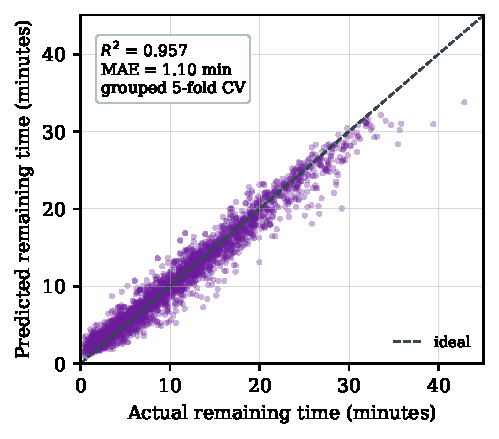
\includegraphics[width=0.82\columnwidth]{fig3_pred_vs_actual.pdf}
\caption{Predicted versus actual remaining drying time for the random
forest under grouped five-fold cross-validation. Each drying profile was
assigned wholly to a single fold; the dashed line denotes ideal
agreement.}
\label{fig3}
\end{figure}

\begin{table}[t]
\caption{Predictive Model Performance (Five-Fold Cross-Validation)}
\begin{center}
\renewcommand{\arraystretch}{1.15}
\footnotesize
\begin{tabular}{@{}llccc@{}}
\toprule
\textbf{Target} & \textbf{Model} & \textbf{$R^{2}$} & \textbf{MAE} &
\textbf{RMSE} \\
\midrule
Remaining time\,\textsuperscript{a} (min) & Random Forest & 0.956 & 1.10 & 1.50 \\
 & Gradient Boosting & 0.950 & 1.23 & 1.61 \\
 & Linear Regression & 0.913 & 1.59 & 2.12 \\
\midrule
Total drying time\,\textsuperscript{b} (min) & Random Forest & 0.924 & 1.37 & 1.78 \\
Recommended temp.\,\textsuperscript{b} (\textdegree C) & Random Forest & 0.567 & 3.53 & 4.43 \\
\bottomrule
\end{tabular}
\label{tab1}
\end{center}
\footnotesize\textsuperscript{a}Grouped cross-validation by drying
profile. \quad
\textsuperscript{b}Pre-drying joint model; per-target metrics from
standard five-fold cross-validation.
\end{table}

\subsection{System Functional Validation}
Table~\ref{tab2} summarises how each function was exercised. The two-phase
start, the re-estimation loop, the risk assessments, the safety clamp and
fault transitions, and the completion/cooling sequence run end-to-end
against the live services and mobile application. The drying-controller
state machine and sensor parser have unit tests, including the one-shot
completion event, the manual heater cut-off, and rejection of malformed
lines. The state-reconciliation fix is confirmed by the client suspending
the countdown whenever the chamber reports it is not running. No function
has yet been validated in field production.

\begin{table}[t]
\caption{System Functional Validation}
\begin{center}
\renewcommand{\arraystretch}{1.12}
\footnotesize
\begin{tabular}{@{}p{2.7cm}p{2.5cm}p{2.2cm}@{}}
\toprule
\textbf{Function} & \textbf{Evidence} & \textbf{Status} \\
\midrule
Remaining-time prediction & Grouped 5-fold test & Integrated;
grouped cross-validation \\
Pre-drying prediction & 5-fold test & Integrated; cross-validated \\
Spoilage-risk rule & Weighted rule + factor breakdown & Integrated;
functionally tested \\
Over-drying auto-stop & Debounced rule issues stop command & Integrated;
functionally tested \\
Two-phase drying start & Chamber sensor check before active-batch record
& Integrated; functionally tested \\
Set-point safety clamp & Bound applied in three places & Integrated;
correct by construction \\
Sensor-fault handling & Bounded consecutive-failure fault; no resume &
Integrated; unit-tested \\
Completion + cooling & Weight/duration criteria; timed cooling &
Integrated; unit-tested \\
State reconciliation & Chamber status suspends countdown & Integrated;
functionally tested \\
Waste \& salt estimation & Per-variety coefficients on batch &
Integrated; domain validation pending \\
Event-level traceability & Per-service logs keyed on batch ID &
Integrated; completeness pending \\
\bottomrule
\end{tabular}
\label{tab2}
\end{center}
\end{table}

\subsection{Discussion}
Two findings matter beyond the architecture. First, predicted parameters
must be constrained by a safety layer independent of the model: separating
the safety envelope from the prediction path means a model error degrades
accuracy but cannot command an unsafe chamber. Second, the component
holding a logical record of an activity must never be treated as
authoritative about whether it is physically occurring; making the device
authoritative removed a class of misleading displays. Prototype experience
also shows integration benefits are contingent on sensing reliability:
intermittent load-cell dropouts repeatedly triggered protective faults
that halted healthy runs, because both time predictors and the completion
check share the weight signal. Whether multi-modal information provides
value unavailable from single-mode processing is a question for the field
trial below.

\section{Limitations and Future Work}
The drying-time models are cross-validated on a modelled dataset and not
yet tested on independent logged real drying runs; that evaluation, split
at the drying-run level, is the primary pending experiment. Weight
reduction indicates drying progression but is not equivalent to
laboratory-measured moisture content without validation, and $k$, the
gas-to-smell mapping, the alert thresholds, and the temperature envelope
are configurable engineering parameters rather than established constants.
The edge protocol does not yet read back relay state, so control is
commanded but not actuator-acknowledged. Traceability is per-service and
keyed on a shared identifier; a unified timeline is partial. No baseline
comparison against conventional processing has been conducted, so no claim
of improved quality, reduced spoilage, or reduced drying time is made.
Future work will collect logged real drying runs with reference moisture
measurements across varieties; add actuator acknowledgement and measure
temperature-tracking error, humidity exposure, actuator latency, and
communication success rate; train and evaluate a spoilage classifier;
consolidate the traceability timeline; and run a controlled comparison of
Smart Karawala against conventional processing.

\section{Conclusion}
Smart Karawala is a batch-centric AI and IoT framework that links
machine-learning drying-parameter prediction to an IoT-controlled drying
chamber, keeps an independent safety layer that can override the predictive
path, and retains every decision as an event-level batch history. A
two-phase start returns predicted parameters to the chamber as control
set-points only after the chamber confirms its sensor state. On a
physics-informed modelled dataset the dynamic remaining-time regressor
reached a grouped cross-validated $R^{2}$ of $0.96$ (MAE $1.1$~min), and
the integrated workflow -- prediction, control-profile handoff,
sensor-validated start, live re-estimation, safety auto-stop, completion,
and event logging -- is operational. The framework makes an
experience-dependent process measurable and traceable; quantifying its
benefit over conventional processing is the immediate next step.

\section*{Acknowledgment}
The authors thank their academic supervisors, domain experts, and the
dry-fish processors who supported this work.

\begin{thebibliography}{00}
\bibitem{b1} N. Mishra, S. K. Jain, N. Agrawal, N. K. Jain, N. Wadhawan,
and N. L. Panwar, ``Development of drying system by using internet of
things for food quality monitoring and controlling,'' \textit{Energy
Nexus}, vol. 11, art. 100219, Sep. 2023, doi: 10.1016/j.nexus.2023.100219.
\bibitem{b2} Y. Alvinika, D. B. Setyohadi, and M. Sulistyoningsih,
``IoT-based monitoring and design of automatic fish drying equipment using
fuzzy logic,'' \textit{IOP Conf. Ser.: Earth Environ. Sci.}, vol. 704, no.
1, art. 012042, 2021, doi: 10.1088/1755-1315/704/1/012042.
\bibitem{b3} J. Guo \textit{et al.}, ``Intelligent monitoring, predicting,
and control technology of food drying: recent advances, challenges, and
future prospects,'' \textit{Food Control}, vol. 180, art. 111666, 2026,
doi: 10.1016/j.foodcont.2025.111666.
\bibitem{b4} R. Rakholia, A. L. Su\'{a}rez-Cetrulo, M. Singh, and R. S.
Carbajo, ``AI-driven meat food drying time prediction for resource
optimization and production planning in smart manufacturing,''
\textit{IEEE Access}, vol. 13, pp. 22420--22428, 2025,
doi: 10.1109/ACCESS.2025.3534379.
\bibitem{b5} F. Ahmad, M. S. Younis, R. U. Zahid, and L. A. Shahid,
``Machine learning based grain moisture estimation for real-time
monitoring of high-temperature paddy drying silo,'' in \textit{Proc. IEEE
23rd Int. Multitopic Conf. (INMIC)}, 2020, pp. 1--6,
doi: 10.1109/INMIC50486.2020.9318092.
\bibitem{b6} T. H. M. Ghanem \textit{et al.}, ``Thin-layer modeling,
drying parameters, and techno-enviro-economic analysis of a solar dried
salted tilapia fish fillets,'' \textit{Sci. Rep.}, vol. 15, art. 5073,
2025, doi: 10.1038/s41598-025-87807-w.
\bibitem{b7} J. H. Friedman, ``Greedy function approximation: a gradient
boosting machine,'' \textit{Ann. Statist.}, vol. 29, no. 5, pp.
1189--1232, 2001, doi: 10.1214/aos/1013203451.
\bibitem{b8} M. R. M. Setyagraha, H. A. Nurqamaradillah, L. M. Hermawan,
N. R. Pratama, L. Novamizanti, and D. R. Wijaya, ``A portable real-time
electronic nose for evaluating seafood freshness using machine learning,''
\textit{IEEE Access}, vol. 13, pp. 82000--82019, 2025,
doi: 10.1109/ACCESS.2025.3576345.
\bibitem{b9} L. Breiman, ``Random forests,'' \textit{Mach. Learn.}, vol.
45, no. 1, pp. 5--32, 2001, doi: 10.1023/A:1010933404324.
\bibitem{b10} J. Cromwell, C. Turkson, M. Dora, and F. A. Yamoah,
``Digital technologies for traceability and transparency in the global
fish supply chains: a systematic review and future directions,''
\textit{Marine Policy}, vol. 178, art. 106700, Aug. 2025,
doi: 10.1016/j.marpol.2025.106700.
\bibitem{b11} Y. P. Tsang, K. L. Choy, C. H. Wu, G. T. S. Ho, and H. Y.
Lam, ``Blockchain-driven IoT for food traceability with an integrated
consensus mechanism,'' \textit{IEEE Access}, vol. 7, pp. 129000--129017,
2019, doi: 10.1109/ACCESS.2019.2940227.
\bibitem{b12} Food and Agriculture Organization of the United Nations,
``Postharvest losses in the multiday fisheries sector of Sri Lanka,'' FAO,
Rome, Italy, 2021.
\end{thebibliography}

\end{document}
